58. \begin{figure}[ht!]
\center{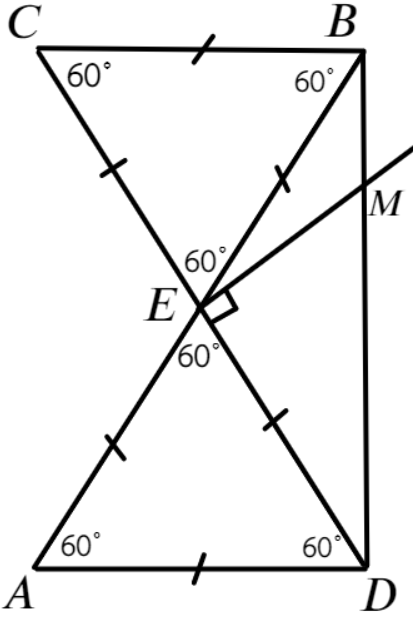
\includegraphics[scale=0.35]{g58.png}}
\end{figure}\\
Так как отрезки $AB$ и $CD$ равны и пересекаются в середине, $AE=BE=CE=DE.$ Так как $AD=CE=AE=DE,$ треугольник $AED$ является равносторонним, а значит $\angle AED=60^\circ=\angle BEC,$ значит треугольник $BEC$ также является равносторонним. Равные углы $BCE$ и $EDA$ являются накрест лежащими, значит прямые $BC$ и $AD$ параллельны, поэтому $\angle CBD+\angle ADB=180^\circ$ (они односторонние). $\left.\begin{array}{l}BC=AD,\\
CD=AB,\\
\angle BCD=\angle DAB  \end{array}
ight\}\Rightarrow \Delta BCD=\Delta DAB\text{ по I признаку}\Rightarrow \angle CBD=\angle ADB.$ Так как $\angle CBD+\angle ADB=180^\circ,$ получаем $\angle CBD=\angle ADB=90^\circ.$ Это значит, что $MB\perp BC,$ то есть длина $BM$ и является расстоянием от точки $M$ до прямой $BC.$ Найдём $\angle EBM=90^\circ-60^\circ=30^\circ.$ Также и $\angle BEM=90^\circ-60^\circ=30^\circ.$ Поэтому треугольник $BEM$ является равнобедренным и $BM=EM.$ Теперь найдём $\angle MDE=90^\circ-60^\circ=30^\circ.$ В прямоугольном треугольнике $EMD$ катет $EM$ лежит напротив угла в $30^\circ,$ а значит $MD=2EM=2BM,$ ч.т.д.\\
